\section{Implementacja}
\subsection{Budowa terenu}\label{subsec:budowa_terenu}
Budowa podstawowej mapy gry jest stosunkowo nieskomplikowanym procesem, dzięki czemu mogliśmy się tutaj skupić głównie na projektowaniu dróg, rozłożeniu obiektów i kształtowaniu mapy na potrzeby rozgrywki.

\paragraph{Przygotowanie terenu}

    Do przygotowania terenu został użyty specjalnie do tego przeznaczony typ obiektu 3D o nazwie \name{Terrain}. Po utworzeniu takiego obiektu w hierarchii obiektów na ekranie ukaże się nieoteksturowana płaszczyzna.

    \begin{figure}[H]
    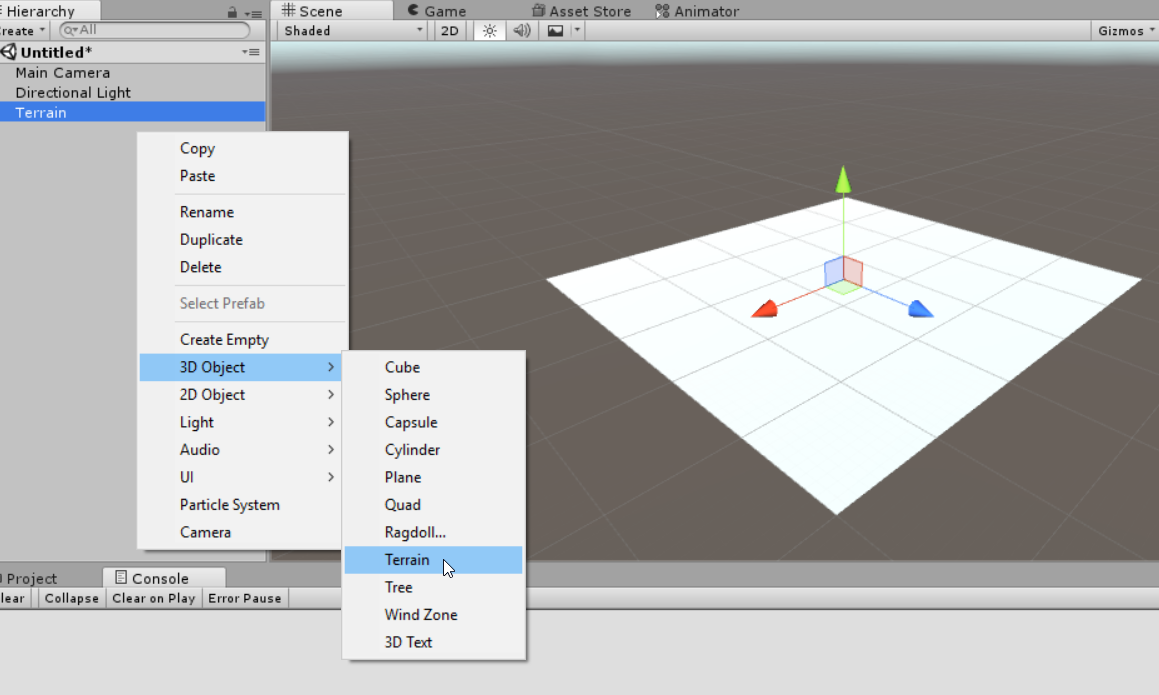
\includegraphics[width=\textwidth]{teren_1.png}
    \caption{Płaszczyzna terenu}
    \end{figure}

\paragraph{Formowanie kształtu} 

    Na tak przygotowanej płaszczyźnie uformowane zostały nierówności przy użyciu palety narzędzi terenu. Używając opcji \name{Raise / Lower Terrain} utworzone zostały wypiętrzenia nadające kształt mapie gry. Charakter wypiętrzeń dostosowany został używając odpowiedniego pędzla z panelu \name{Brushes}, natomiast promień zniekształceń oraz siła efektu za pomocą parametrów kolejno \name{Brush Size} oraz \name {Opacity}.

    \begin{figure}[H]
    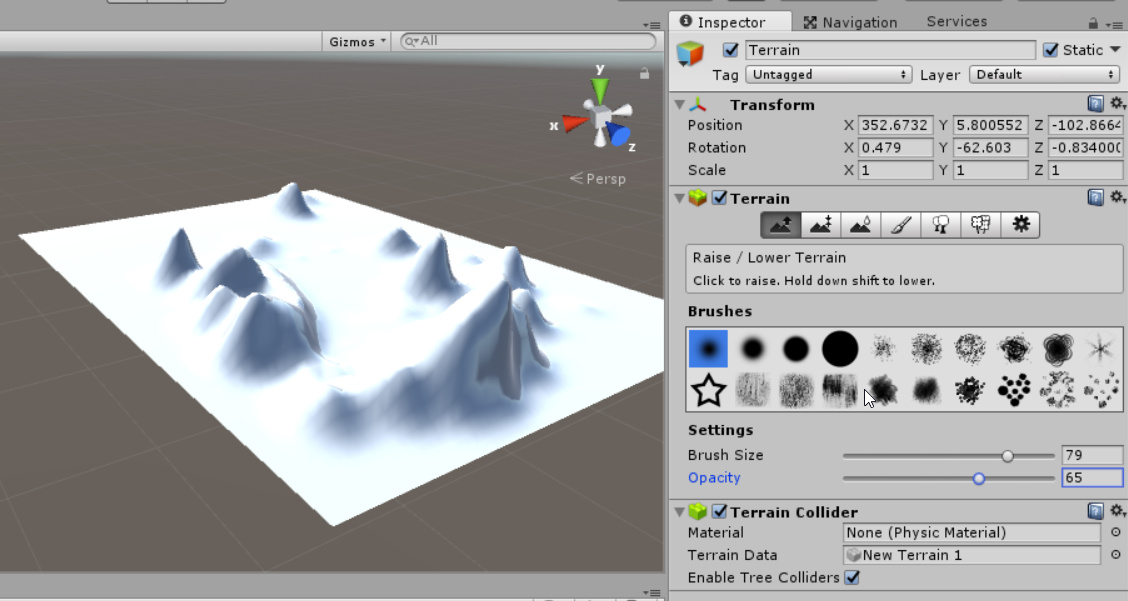
\includegraphics[width=\textwidth]{teren_2.png}
    \caption{Modelowanie nierówności terenu}
    \end{figure}

\paragraph{Nakładanie tekstur}

    Kolejnym krokiem było utworzenie tekstury służącej do nadaniu naszemu terenowi koloru oraz faktury. Do tego celu pobrane zostały odpowiednie tekstury z wbudowanego sklepu assetów \name{Asset Store}. Assety są rodzajem pakietów zawierających różnorakie obiekty, skrypty oraz tekstury, dostępne do pobrania z serwerów Unity.

    Po pobraniu odpowiedniej tekstury trawy, zostaje ona zaimportowana do folderu \name{Assets} znajdującego się w głównym katalogu projektu.

    Po wybraniu narzędzia \name{Paint Texture} ukazuje się panel \name{Textures} pozwalający na skonfigurowanie używanej przez narzędzie tekstury. Znajduje się tam przycisk \name{Edit Textures...} po kliknięciu którego otwiera się okno konfiguracyjne tekstury pozwalające na wybór tekstury podstawowej oraz tekstury przechowującej dane o chropowatościach. Po skonfigurowaniu tekstur i nałożeniu ich na teren, całość prezentuje się następująco.

    \begin{figure}[H]
    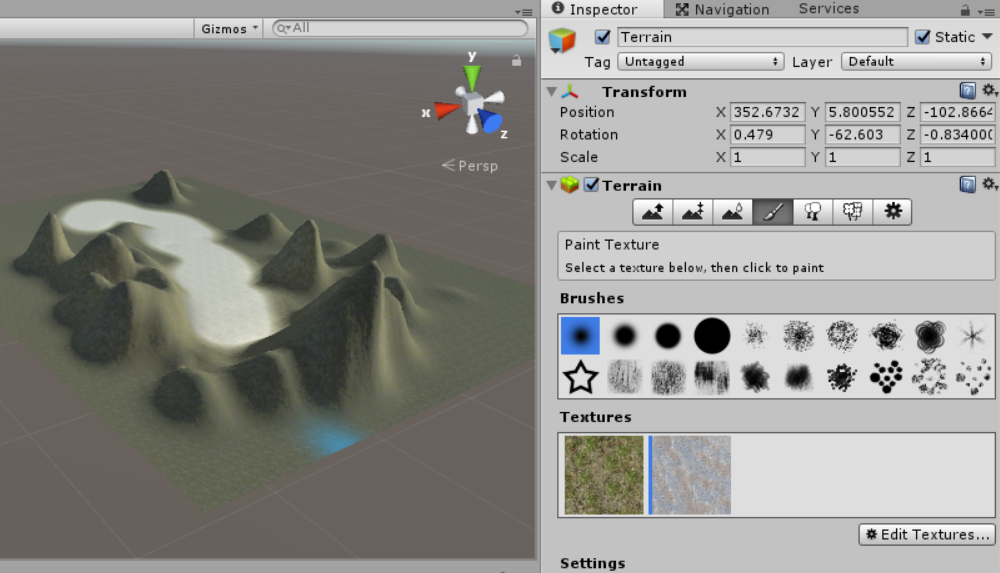
\includegraphics[width=\textwidth]{teren_3.png}
    \caption{Nakładanie tekstur na mapę terenu}
    \end{figure}

\paragraph{Rozmieszczanie obiektów}

    Kolejnym krokiem w tworzeniu świata gry było umieszczenie na mapie sprefabrykowanych wcześniej obiektów (tzw. \textit{Prefabs}, o tym później). Wszystkie obiekty użyte w pracy są dostępne za darmo w bibliotece obiektów Unity (\name{Asset Store}). Po pobraniu, obiekty znajdują się w podfolderze \name{Prefabs} zainstalowanej paczki. Obiekty umieszcza się na mapie metodą przeciągnij-upuść, dostosowując ich koordynaty używając narzędzi transformacji dostępnych w pasku narzędzi znajdującym się w górnej części okna edytora.

    \begin{figure}[H]
    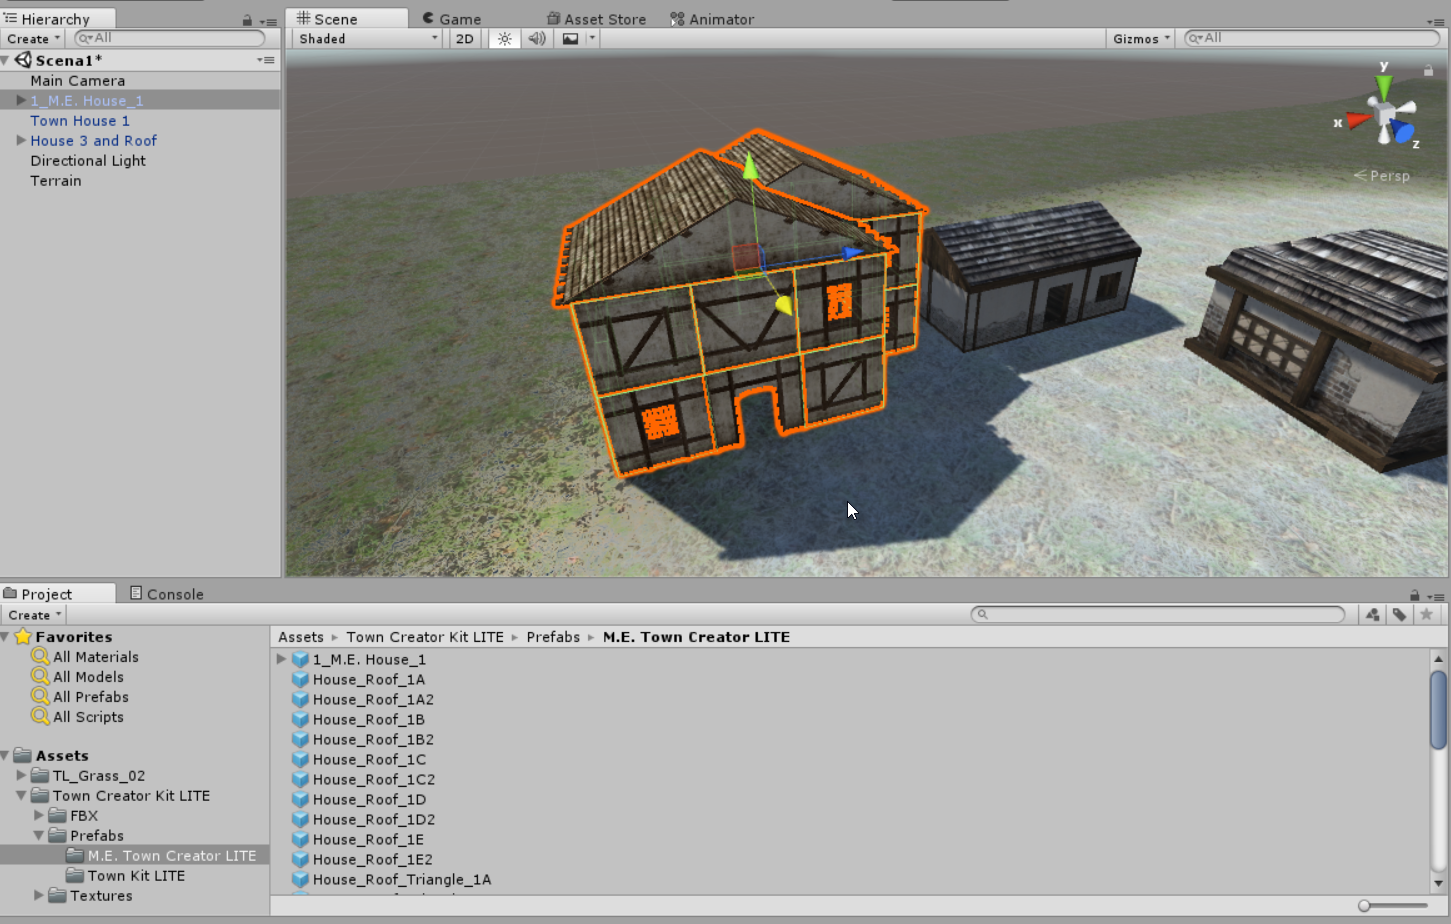
\includegraphics[width=\textwidth]{teren_obiekty.png}
    \caption{Umieszczanie obiektów na mapie}
    \end{figure}

    % Szczegóły kolizji w sekcji~\ref{subsec:fizyka} na stronie~\pageref{subsec:fizyka}

\paragraph{Oddziaływanie terenu na inne obiekty}

    Kluczowym elementem tworzenia mapy świata gry są takie elementy jak oddziaływanie na postacie ograniczeń nachylenia terenu typu wzgórza, drzewa, czy budynki, uniemożliwiających dostanie się w niektóre miejsca. Unity w celu uproszczenia obliczeń posiada możliwość wygenerowania uproszczonej mapy dróg (tzw. \textit{NavMesh}) na bazie modelu terenu, pozwalającej na dynamiczne omijanie przeszkód przez wroga (o tym później w sekcji \ref{subsec:poruszanie_wrogow} na stronie \pageref{subsec:poruszanie_wrogow}).

    Aby utworzyć taką mapę, należy przejść do zakładki \name{Navigation}, gdzie w panelu \name{Bake} znajduje się lista parametrów dotyczących maksymalnego kąta nachylenia terenu, czy maksymalnej wysokości uskoku, którą obiekty sterowane przez komputer mogą pokonać.

    \begin{figure}[H]
    \center
    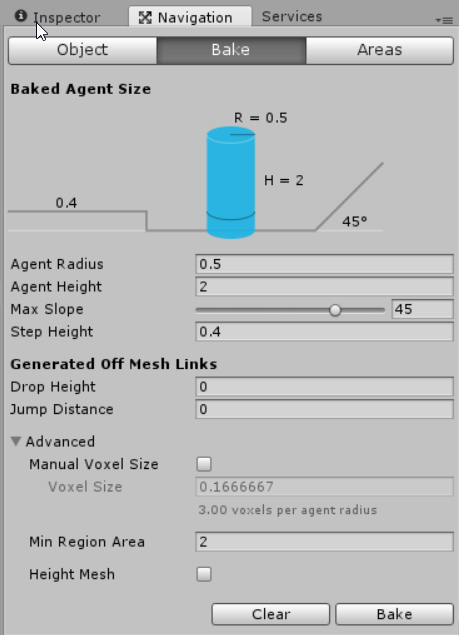
\includegraphics[width=6cm]{teren_obiekty2.png}
    \caption{Parametry mapy dróg}
    \end{figure}

    Po ustaleniu parametrów i kliknięciu przycisku \name{Bake}, mapa zostaje wygenerowana, natomiast w oknie widoku sceny, obszary dostępne do przemierzania oznaczone zostają niebieskim kolorem. Operację można powtarzać do uzyskania optymalnych efektów.

    \begin{figure}[H]
    \center
    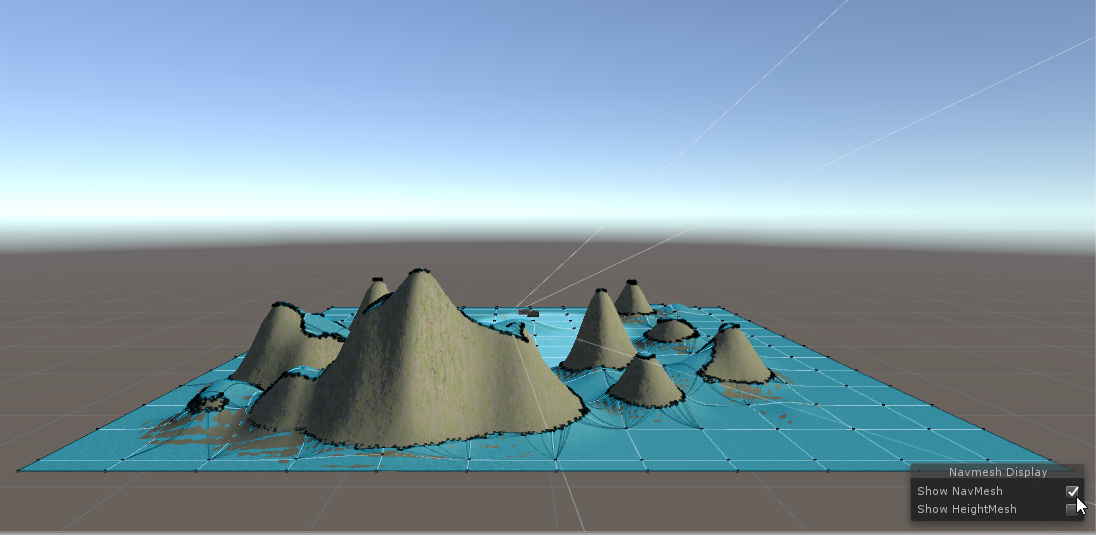
\includegraphics[width=9cm]{teren_obiekty3.png}
    \caption{Poprawnie wygenerowany \textit{NavMesh}}
    \end{figure}

    Tak przygotowana mapa posłużyła nam do projektowania dalszej części gry.

    % Każdy obiekt utworzony w Unity posiada paletę komponentów. Komponenty pozwalają na określanie właściwości obiektów, takich jak rozmiar, pozycja, czy masa. Komponentami są również skrypty, pozwalające na określenie interacji obiektu z zewnętrznym światem (np. zdarzenie \textit{OnCollisionEnter}).